\documentclass[border=3pt,tikz]{standalone}
\usepackage{amsmath}
\usetikzlibrary{calc}
\usetikzlibrary{arrows.meta} % for arrow size
\begin{document}
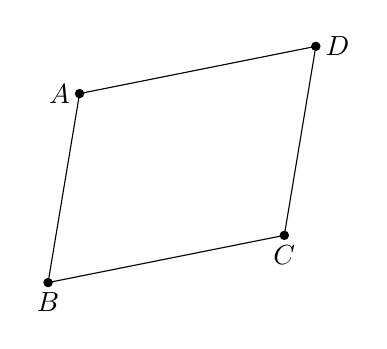
\begin{tikzpicture}[scale=2]
\usetikzlibrary {arrows.meta}
\usetikzlibrary {calc}

\coordinate (A) at (0,0);
\coordinate (D) at (1.5,0.3);
\coordinate (B) at (-0.2, -1.2);
\coordinate (C) at (1.3, -0.9);
\draw[black] (A) -- (D);
\draw[black] (A) -- (B);
\draw[black] (B) --(C);
\draw[black] (D) -- (C);
\fill[black] (A) circle (0.03cm) node[left] {$A$};
\fill[black] (D) circle (0.03cm) node[right] {$D$};
\fill[black] (B) circle (0.03cm) node[below] {$B$};
\fill[black] (C) circle (0.03cm) node[below] {$C$};


\end{tikzpicture}
\end{document}